\section{System Health Management}
\label{sec:shm}

A typical contemporary SHM integration approach is shown in Figure \ref{fig:system}. A DM subsystem generates an action $a_{t,\text{DM}}$, aimed at achieving the operational objectives. The plant executes $a_{t,\text{DM}}$ and an observation $o_t$ is generated and relayed to both DM and SHM. DM computes $a_{t+1,\text{DM}}$ on the basis of $o_t$, while SHM analyzes $o_t$ for indications of \textbf{faults} (defined here as system states considered to be off-nominal) and, if any are detected, issues a mitigation or recovery command $a_{t+1,\text{SHM}}$ either directly to the plant or as a recommendation to the DM subsystem \cite{Valasek2012}.

\begin{figure}[ht]
	\centering
		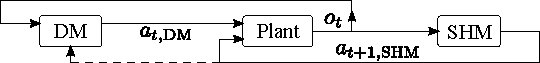
\includegraphics[width=\columnwidth]{figures/system_horizontal.pdf}
	\caption{A typical system architecture with SHM}
	\label{fig:system}
\end{figure}

\begin{figure*}[ht!]
	\centering
		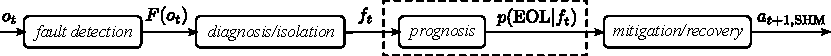
\includegraphics[width=0.9\textwidth]{figures/ishm_horizontal.pdf}
	\caption{A typical contemporary SHM architecture}
	\label{fig:shm}
\end{figure*}

Figure \ref{fig:shm} goes into more detail on the SHM subsystem. The fault detection module corresponds to the traditional red-line monitors detecting threshold-crossing events of sensor values, represented on the diagram by a Boolean \textbf{fault detection} function $F$. If a fault is detected ($F(o_t) = \text{true}$), \textbf{fault isolation} and \textbf{diagnosis} (or \textbf{identification}) is performed, generating a vector of fault descriptors $f_t$ \cite{Daigle2010}. Each fault descriptor typically identifies a component, its fault mode, and its fault parameters \cite{Daigle2010}. There are diagnostic systems that also include an estimated fault probability in the descriptor \cite{Narasimhan2007}. If the uncertainty of the diagnostic results is deemed too high (\textit{e.g.}, $f_t$ consists of only low-probability elements), \textbf{uncertainty management} is sometimes performed in order to obtain a better estimate of the current system condition \cite{Lopez2010}.

Some recent SHM implementations then pass $f_t$ to a \textbf{prognostic} module \cite{Roychoudhury2011}. In the SHM context, the intended goal of the prognostic module is to predict, at time $t_p$ (here $t_p=t$), whether and when faults will lead to system \textbf{failure} (defined as inability to perform its assigned function) within the window $[t_p,t_p+H]$ of a prediction horizon $H$ (the terms \textit{prediction horizon} and \textit{decision horizon} are equivalent for our purposes). In prognostics literature, the time of failure is commonly synonymous with the term \textbf{end of [useful] life (EOL)}. Equivalently, the goal of prognostics can be defined as predicting the system's \textbf{remaining useful life (RUL)}. In Figure \ref{fig:shm}, the prognostic prediction is represented  as a probability distribution $p(\text{EOL}|f_t)$ for $\text{EOL} \in [t_p,t_p+H]$. Uncertainty management is sometimes also prescribed following prognostic analysis, meant to improve the prediction if the confidence in it is insufficiently high \cite{Wang2012}. Note that if a prognostic module is part of an SHM sequence, the term \textbf{Prognostics and Health Management (PHM)} is used by some instead of SHM in order to emphasize the role prognostics is playing in managing the system's lifecycle.

Finally, $p(\text{EOL}|f_t)$ and $f_t$ are passed to the \textbf{fault mitigation and recovery} component to select an action $a_{t+1,\text{SHM}}$ from the action set $A_{\text{SHM}}$, in order to mitigate or recover from faults in $f_t$. As part of this process, operational constraints may be set for those faulty components that cannot be restored to nominal health. If functional redundancy exists for such components, their further use may be avoided.

The overall limitations of the current SHM approach are discussed in Section \ref{sec:hadm}, where an approach that unifies DM and SHM is then proposed. The next section, however, focuses on the prognostic component and discusses why it is not meaningful for actively controlled systems and is challenging to implement in a useful manner for uncontrolled systems.

 



